\section{Reconstructing the hidden geometry from answers}
\label{sec:geom-results}
We first test the reconstruction where the truth is visible: on open models, whose hidden states we store.
\textbf{Data.} 4{,}800 contexts of six kinds (3{,}360 development, 1{,}440 confirmation). Two more sets of 1{,}000 fresh contexts add four new kinds: news, programming, jailbreaks and prompt injections. We ask 88 questions about the message, on eight open chat models from six families. The ground truth is each model's residual stream at the last prompt token, at a layer chosen on development data. All results are on held-out contexts (\cref{app:details}).

\begin{table}[t]
\centering\footnotesize
\renewcommand{\arraystretch}{1.12}
\setlength{\tabcolsep}{2.4pt}
\caption{\textbf{Which observable carries the state?} Spearman correlation of each geometry with the model's own hidden geometry, over all pairs of 1{,}440 held-out contexts; no parameter is fit. Answers: Fisher--Rao distances over 88 questions, exact (log-probabilities) or from 8 answers sampled from the model's own probabilities. Replies: mean embedding of 8 sampled replies. Text: embedding of the input. Last column: answers $-$ text, 95\% interval.}
\label{tab:geometry}
\begin{tabular}{@{}l>{\columncolor{gbrow}}cc cc l@{}}
\toprule
 & \multicolumn{2}{c}{\textbf{Answers}} & & & \\
\cmidrule(lr){2-3}
\textbf{Model} & exact & 8 samples & \textbf{Replies} & \textbf{Text} & \textbf{answers $-$ text}\\
\midrule
\GTABLE
\bottomrule
\end{tabular}
\end{table}

\begin{figure}[t]
\centering
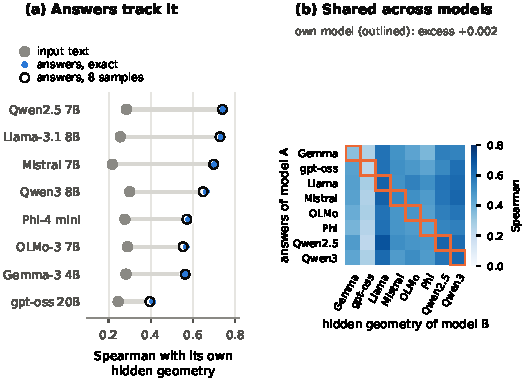
\includegraphics[width=\columnwidth]{figures/geometry_main.pdf}
\caption{\textbf{What yes/no answers reveal of a hidden state} (preregistered). (a) Agreement of each open model's answer geometry with its own hidden geometry, exact and from 8 sampled answers, against the geometry of the input text (Spearman over all pairs of 1{,}440 held-out contexts; nothing fit). (b) Answers of model A against the hidden geometry of model B on 1{,}000 fresh contexts: the own-model diagonal (outlined) is not special.}
\label{fig:geometry}
\end{figure}

\textbf{Answers beat the input and the replies.} On every model, the answer geometry matches the hidden geometry better than a sentence embedding of the input does (gains \GOneGain; every lower bound at least \GOneGainLow; \cref{tab:geometry}). The model's own replies, the other output that an API gives, do little better than the input (\GFiveRep). Agreement rises with the number of questions (from 8 to 88: \GOneMore). Eight sampled answers per question keep \GOneKeep\ of the exact agreement. Given the kind of context, the answers keep a partial Spearman of 0.46 and the input embedding 0.09 (exploratory).

\textbf{The geometry is shared across models.} A model's answers match another model's hidden geometry as well as its own. On 1{,}000 fresh contexts, the mean own-model excess is \GSixExcess, inside the equivalence band of $\pm0.02$ that we fixed in advance (\cref{fig:geometry}b). The hidden geometries of different models also agree with each other (\GSixHH). So the answers reveal the geometry that models share, in line with converging representations \citep{huh2024platonic,picozzi2026information}.

\textbf{A closed model's answers are reliable.} Claude Haiku 5.5 answered 24 questions, 8 times each, on 192 held-out contexts. Two independent halves of its answers give the same geometry (Spearman \GTwoSplit; bound fixed in advance: 0.7). This geometry carries \GTwoText\ beyond the input embedding.

\textbf{Triangulation estimates a closed model's own agreement.} Its hidden states are not visible, so we triangulate through the shared geometry (\cref{prop:triang}). We first test the estimator on open models. We leave each open model out, as if it were closed, with its answers sampled to the closed design. The estimate then predicts its true agreement to within \GVtMae\ on average (\GVtInside\ of 8 inside the predicted interval). For Claude Haiku 5.5 the estimate is \GVtClosed. This is at the level of its direct agreement with open models' hidden geometries (0.45--0.51) and at the bottom of the open range (\GVtOpenRange). The estimate assumes no own-model excess, as found above; over the range of open-model loadings, its interval is [0.32, 0.53].

% =====================================================================================
\section{Monitoring, forecasting and preventing violations}
\label{sec:results}
\textbf{Agents and benchmarks.} CAPE-Bench \citep{fayyazi2026cape} gives matched tool-use tasks in which one fact decides whether an action is authorised. An environment checker labels each action. We use four open agents, whose decision states we store: Gemma-4 (26B), gpt-oss-20b, Qwen3.8-27B and Muse-Glimmer-30B. We use two closed agents through their public APIs, with reasoning off: Claude Haiku 5.5 (Anthropic) and GPT-6-luna (OpenAI). The second benchmarks are AgentDojo (prompt injection) and $\tau^2$-bench airline.

\subsection{Monitoring at the call}
\label{sec:monitor}
\textbf{The read-out.} At each proposed call, the agent answers 8 yes/no questions about the call through its own API, 4 times each. The fixed read-out of \cref{sec:method} scores the answers. Nothing is fit and no label is used: we fixed the questions and the read-out on development data.

\textbf{It ranks violations about as well as a probe on the hidden states.} On held-out calls, the within-template AUROC is \GFtFixed\ (\cref{tab:g15}). A probe trained on the agent's true decision states, a comparison that needs the weights and labels, scores \GFtTrainedWB; the mean difference is \GFtTtwo. The read-out beats the agent's single self-audit answer by \GFtTone. The 8 answers measure a narrow slice of the decision state: their geometry agrees with the full state at only 0.01--0.16. It is the slice that bears on the violation.

\textbf{It beats a reasoning judge on open agents.} Gemma-4, with reasoning on, read each conversation and gave one holistic violation probability. It ranked the open agents' violations worse than the read-out (read-out $-$ judge \GTwJone; two-sided test). Fixed questions and averaged angles beat one verdict. On Claude Haiku 5.5's actions, which it answered with its reasoning off, the judge is better (\cref{tab:g15}).

\begin{table}[t]
\centering\footnotesize
\setlength{\tabcolsep}{3pt}
\caption{\textbf{Monitoring a decision through the agent's own answers} (preregistered; held-out calls). Within-template AUROC (within tool on $\tau^2$-bench; the Claude Haiku 5.5 ``all'' row is pooled). The read-out of 8 answers is fixed (nothing fit to labels). The trained probe reads the agent's true hidden states (32 principal components, fit on development calls); it is a comparison, not part of the method.}
\label{tab:g15}
\resizebox{\columnwidth}{!}{\begin{tabular}{@{}l c ccccc@{}}
\toprule
Agent & calls & \textbf{8 answers} & 1 answer & judge\textsuperscript{d} & trained & tuned\textsuperscript{c}\\
\midrule
Gemma-4 (new task families) & 600 & \textbf{0.994} & 0.966 & 0.989 & 0.980 & 0.991\\
gpt-oss-20b & 599 & 0.822 & 0.758 & 0.755 & 0.772 & \textbf{0.841}\\
Qwen3.8-27B & 373 & \textbf{0.951} & 0.894 & 0.780 & 0.826 & 0.950\\
Muse-Glimmer-30B & 600 & 0.929 & 0.935 & 0.880 & 0.941 & \textbf{0.972}\\
\midrule
Claude Haiku 5.5, restarts\textsuperscript{a} & 149 & 0.909 & 0.323 & \textbf{1.000} & -- & --\\
Claude Haiku 5.5, all\textsuperscript{b} & 495 & 0.475 & 0.306 & \textbf{0.693} & -- & --\\
GPT-6-luna & 560 & \textbf{0.979} & 0.795 & -- & -- & --\\
\midrule
\multicolumn{7}{@{}l}{\emph{Second benchmarks: AgentDojo (within suite), $\tau^2$-bench airline (within tool)}}\\
Gemma-4, prompt injection & 816 & \textbf{0.985} & 0.975 & -- & -- & --\\
gpt-oss-20b, prompt injection & 821 & \textbf{0.904} & 0.900 & -- & -- & --\\
Claude Haiku 5.5, airline writes & 360 & \textbf{0.704} & 0.555 & -- & -- & --\\
\bottomrule
\end{tabular}}\\[2pt]
\parbox{\columnwidth}{\scriptsize \textsuperscript{a}Closed: no trained probe exists; a trained reader of the call text scores 1.000 here. \textsuperscript{b}Pooled; its mailing-list sends are decided by a fact that it never checked, and they are not flagged. \textsuperscript{c}Exploratory: a probe on the true states, with its components and regularisation chosen afterwards by cross-validation on the development calls. \textsuperscript{d}Gemma-4 with reasoning on reads the same conversation and gives one holistic violation probability (mean of 4).}
\end{table}

\textbf{With no label, the read-out tells where it works.} Its variance beyond its known sampling noise is its SNR (\cref{prop:snrceil}). Over \GCwCells\ agent--benchmark--stratum cells, the SNR predicts the AUROC (Spearman \GCwCone): cells with SNR $>0$ score \GCwPos, and cells with SNR $\le0$ score \GCwNeg. The same holds for each question: over eight agent--benchmark pairs, a question's label-free spread beyond its noise predicts how well it ranks violations (mean Spearman \GTfFone). Claude Haiku 5.5's settings have the lowest SNR: its four answers agree on 96--97\% of questions.

\textbf{At the call, another answerer does as well.} On open agents, another model that answers the same questions about the same call does about as well (own $-$ other +0.012 [$-$0.018, 0.040]). On Claude Haiku 5.5 it does better ($-$0.09 on restarts; $-$0.29 on $\tau^2$, with reasoning on). The theory predicts this parity. At the call, the transcript and the call decide the violation (\cref{cor:action}), so any capable reader of them can match the agent. The agent's own state matters before the call (\cref{sec:forecast}).

\subsection{Carrying to new benchmarks and closed agents}
\label{sec:carry}
\textbf{Prompt injection.} On AgentDojo \citep{debenedetti2024agentdojo}, the violation is a call that carries out an instruction hidden in a tool output. We wrote 8 questions from that policy before any answer existed. The same read-out ranks the open agents' injected calls within suite, on held-out tasks with no defense, at \GSvGemma\ (Gemma-4, \GSvGemmaN) and \GSvGpt\ (gpt-oss-20b, \GSvGptN); the bar was a lower bound above 0.60. Here the single overall question is nearly as good (difference \GSvVtwo). Claude Haiku 5.5 almost never carried out these injections (none in 271 development episodes), so this benchmark has no closed-agent arm.

\textbf{GPT-6-luna.} Through its own API, its answers to the same 8 questions rank its CAPE-Bench violations within template and tool at \GGlAt\ (\GGlN). Its single answer scores 0.795.

\textbf{Claude Haiku 5.5 on CAPE-Bench.} The read-out ranks its unapproved restarts at \GFtClosedAFixed, where its single self-audit answer scores 0.32. Pooled over all its actions, the read-out scores 0.475: a fact that the agent never checked decides its mailing-list sends, so its state holds no warning about them.

\textbf{Claude Haiku 5.5 on $\tau^2$-bench.} On $\tau^2$-bench airline \citep{barres2025tau2}, Claude Haiku 5.5 breaks the published policy at some of its writes; for example, it cancels a booking that meets none of the conditions. We wrote 8 questions from the airline policy before any answer existed. The within-tool AUROC is \GEeRone\ (\GEeN, in 7 tasks; bar: lower bound above 0.5), and its single answer to whether the call complies scores \GEeSingle. With 5\% of writes reviewed, the read-out catches \GEeCaught. Per task (exploratory), it ranks the violations of 5 of the 7 tasks (33 of 50) at 0.77--1.00. In the other two tasks, the agent made an honest mistake: its own reply called the write eligible (it missed a flown date; it reversed a trip). Its state held no warning to read.

\subsection{Forecasting before the call}
\label{sec:forecast}
\textbf{The pre-call state.} Before each step's call, the agent answers 8 questions about its next action. The call is not shown, because it does not exist yet.

\textbf{GPT-6-luna's state forecasts the coming violation.} Its pre-call answers rank the coming violation at \GGlPre. Pooled, this equals position alone (\GGlPos). Among calls at the same position, where position cannot help, they rank it at \GGlPrePos\ (exploratory). A preregistered replication on \GCfN\ confirms it: \GCfPos.

\textbf{The forecast is the agent's own.} Gemma-4 answered the same questions in GPT-6-luna's seat, on the same conversations. Within each kind of task and tool, it forecast worse: 0.728, against 0.840 for GPT-6-luna's own answers (difference +0.111 [0.041, 0.185]). At the same position, the difference is +0.08 [$-$0.02, 0.23] and does not separate. \Cref{prop:selfforecast} predicts this order: before the call, only the agent's own policy gives the Bayes forecast. On open agents the comparison is mixed (Qwen3.8 +0.21; gpt-oss-20b $-$0.16; Muse-Glimmer $-$0.15).

\textbf{Open agents.} On Gemma-4 (2{,}505 steps of 300 held-out episodes), among calls at the same step of the same kind of task, the pre-call answers rank the violating calls at 0.67 (exploratory). Three more agents confirm it (0.669 [0.594, 0.764]), and 16 answers per question raise it to 0.73. The deciding fact enters at the call's own step: the answers then rank the call better than one step earlier (+0.16 [0.03, 0.30]). The state has a short memory (autocorrelation 0.13 at one step, 0.01 at three). A Kalman forecast from earlier steps beat position on three agents (+0.21 [0.08, 0.32]). It failed on Gemma-4, where the filter assumed a noise about three times too large.

\textbf{Where it does not forecast.} Before Claude Haiku 5.5's $\tau^2$ writes, its answers did not rank the coming violation (0.54 [0.43, 0.68]).

\subsection{Preventing violations}
\label{sec:prevent-live}
\textbf{Self-policing.} Before a non-read call runs, a side branch asks the agent whether the call complies with its policy, and a flagged call goes to review. At one state, a gate prevents the share $\tau$ of violating calls that the agent flags. Over many states, it prevents the mean of $\tau$, weighted by where the violations occur (\cref{prop:prevention}).

\begin{table}[t]
\centering\footnotesize
\renewcommand{\arraystretch}{1.12}
\setlength{\tabcolsep}{2.4pt}
\caption{\textbf{Self-policing through the agent's own API} (preregistered; held-out scenarios; no other model, no labels). Episodes with an executed violation, and episodes that reached the goal without one, in \%; reduction $=1-$gate/plain, 95\% interval.}
\label{tab:selfpolice}
\begin{tabular}{@{}l cc c cc@{}}
\toprule
 & \multicolumn{2}{c}{\textbf{Violations}} & & \multicolumn{2}{c}{\textbf{Success}}\\
\cmidrule(lr){2-3}\cmidrule(lr){5-6}
\textbf{Agent, set} & plain & gate & reduction & plain & gate\\
\midrule
Gemma-4, all\textsuperscript{a} & 27.9 & \textbf{5.0} & .82 {\scriptsize[.76, .88]} & 33.5 & \textbf{43.7}\\
Claude Haiku 5.5, decidable\textsuperscript{b} & 2.8 & \textbf{0.9} & .69 {\scriptsize[.51, .88]} & \multirow{2}{*}{40.4} & \multirow{2}{*}{40.1}\\
Claude Haiku 5.5, unchecked fact\textsuperscript{c} & 100 & 92.9 & .07 {\scriptsize[.00, .17]} & & \\
\midrule
\multicolumn{6}{@{}l}{\textit{AgentDojo: attacks succeeded; utility}}\\
Gemma-4\textsuperscript{d} & 11.5 & \textbf{1.8} & .84 {\scriptsize[.76, .91]} & 84.5 & 86.8\\
gpt-oss\textsuperscript{d} & 24.4 & \textbf{12.2} & .50 {\scriptsize[.42, .58]} & 50.5 & 50.8\\
\bottomrule
\end{tabular}\\[2pt]
\parbox{\columnwidth}{\scriptsize \textsuperscript{a}666 episodes per arm; a call was held when all four answers said that it does not comply (1.01 reviews per episode; reviewer: CAPE's checker). A second gate, which replaces a flagged call by a fresh draw (up to four), also gave $-84\%$, with success 38.7 and 0.40 reviews per episode (its review limit, 0.40, failed). \textsuperscript{b}470 scenarios $\times$ 2; a call was held when all three answers said that it breaks a rule; 0.31 reviews per episode. \textsuperscript{c}21 mailing-list scenarios $\times$ 2; predicted not to fall. \textsuperscript{d}Held-out tasks, 2 trials, about 1{,}300 attacks per arm; spotlighting in both arms; predicted 1.00 and 0.58.}
\end{table}

\textbf{Live results.} On unseen scenarios (\cref{tab:selfpolice}), Gemma-4 prevented 82\% of its violating episodes and reached more goals. Claude Haiku 5.5, asked to check its policy rule by rule, prevented 69\% of the violating episodes that its transcript decides, at no cost in goals. Against prompt injection on AgentDojo, the gate cut attack success by 84\% and 50\%, at no cost in utility.

\textbf{The effect is predictable.} Offline flag rates, weighted by where each agent violates, predicted the live reduction of five agents within the registered 0.15 (reductions from 0.01 to 0.63; mean absolute error 0.035; \cref{fig:teaser}d).

\textbf{A gate on the pre-call state.} We ran GPT-6-luna live, with gates at an equal review rate (\GLbRev\ reviews per episode). A gate on its pre-call read-out cut the episodes with a violation from \GLbNone\ to \GLbPre\ (relative reduction \GLbRed). A gate on position cut them to \GLbPos\ (difference \GLbPmP). Success did not change (\GLbSucc). The offline share of violating calls that the gate holds, fixed before the analysis, predicted its effect (\GLwPred; observed \GLwObs). The same law under-predicted the position gate (0.17 vs 0.44), whose episodes also reached the goal more often (27.8\% vs 18.7\%). On Gemma-4, whose pre-call read-out ranks weakly, the gate did not prevent.

\textbf{Trained comparisons} (\cref{app:trained}). With labels, a probe on an open reader of the transcript is stronger (0.98--0.99 on held-out actions of open and closed agents). But it needs labels for each policy, and it fell to 0.54 on unseen $\tau^2$ tasks. The training-free read-out needs neither, so the two are complementary.
